% The theory and concepts of your work. For example, if you work on compiler you can mention about how compiler works without getting much into detail.

\newcommand{\argmin}{\operatornamewithlimits{arg\,min}}
\newcommand{\Bx}{{\bf x}}
\newcommand{\By}{{\bf y}}
\newcommand{\Bh}{{\bf h}}
\newcommand{\Bw}{{\bf w}}
\newcommand{\Bc}{{\bf c}}

In this section we will describe the basics of artificial neural networks. We will also introduce the notation used in this work. Note that the definitions and notations vary through the literature. We use the one which the author is familiar with. For the reader who is comfortable with this topic we recommend to skip this section and go to related models \ref{overview-models}. 

%=============================================================
\subsubsection{Perceptron.}
\label{sec:models-perceptron}

The theory behind artificial neural networks started with the model of \emph{Perceptron} introduced by~\citet{mcculloch1943logical}. It is a simple model which transforms a vector of inputs $s$ to an output value $y$. The notation as depicted on figure~\ref{fig:perceptron}: $x$ is the \emph{input vector} where always $x_0=1$, $w_{0k}$ is the \emph{weight} vector, $\Sigma$ is the \emph{summing} junction, $\eta_k$ is the \emph{net input}, $\phi$ is the \emph{activation function}, $\theta_k$ is the \emph{treshold}, $y_k$ is the \emph{output} and $b_k$ is the \emph{bias}.

\begin{figure}[H]
  \centering
  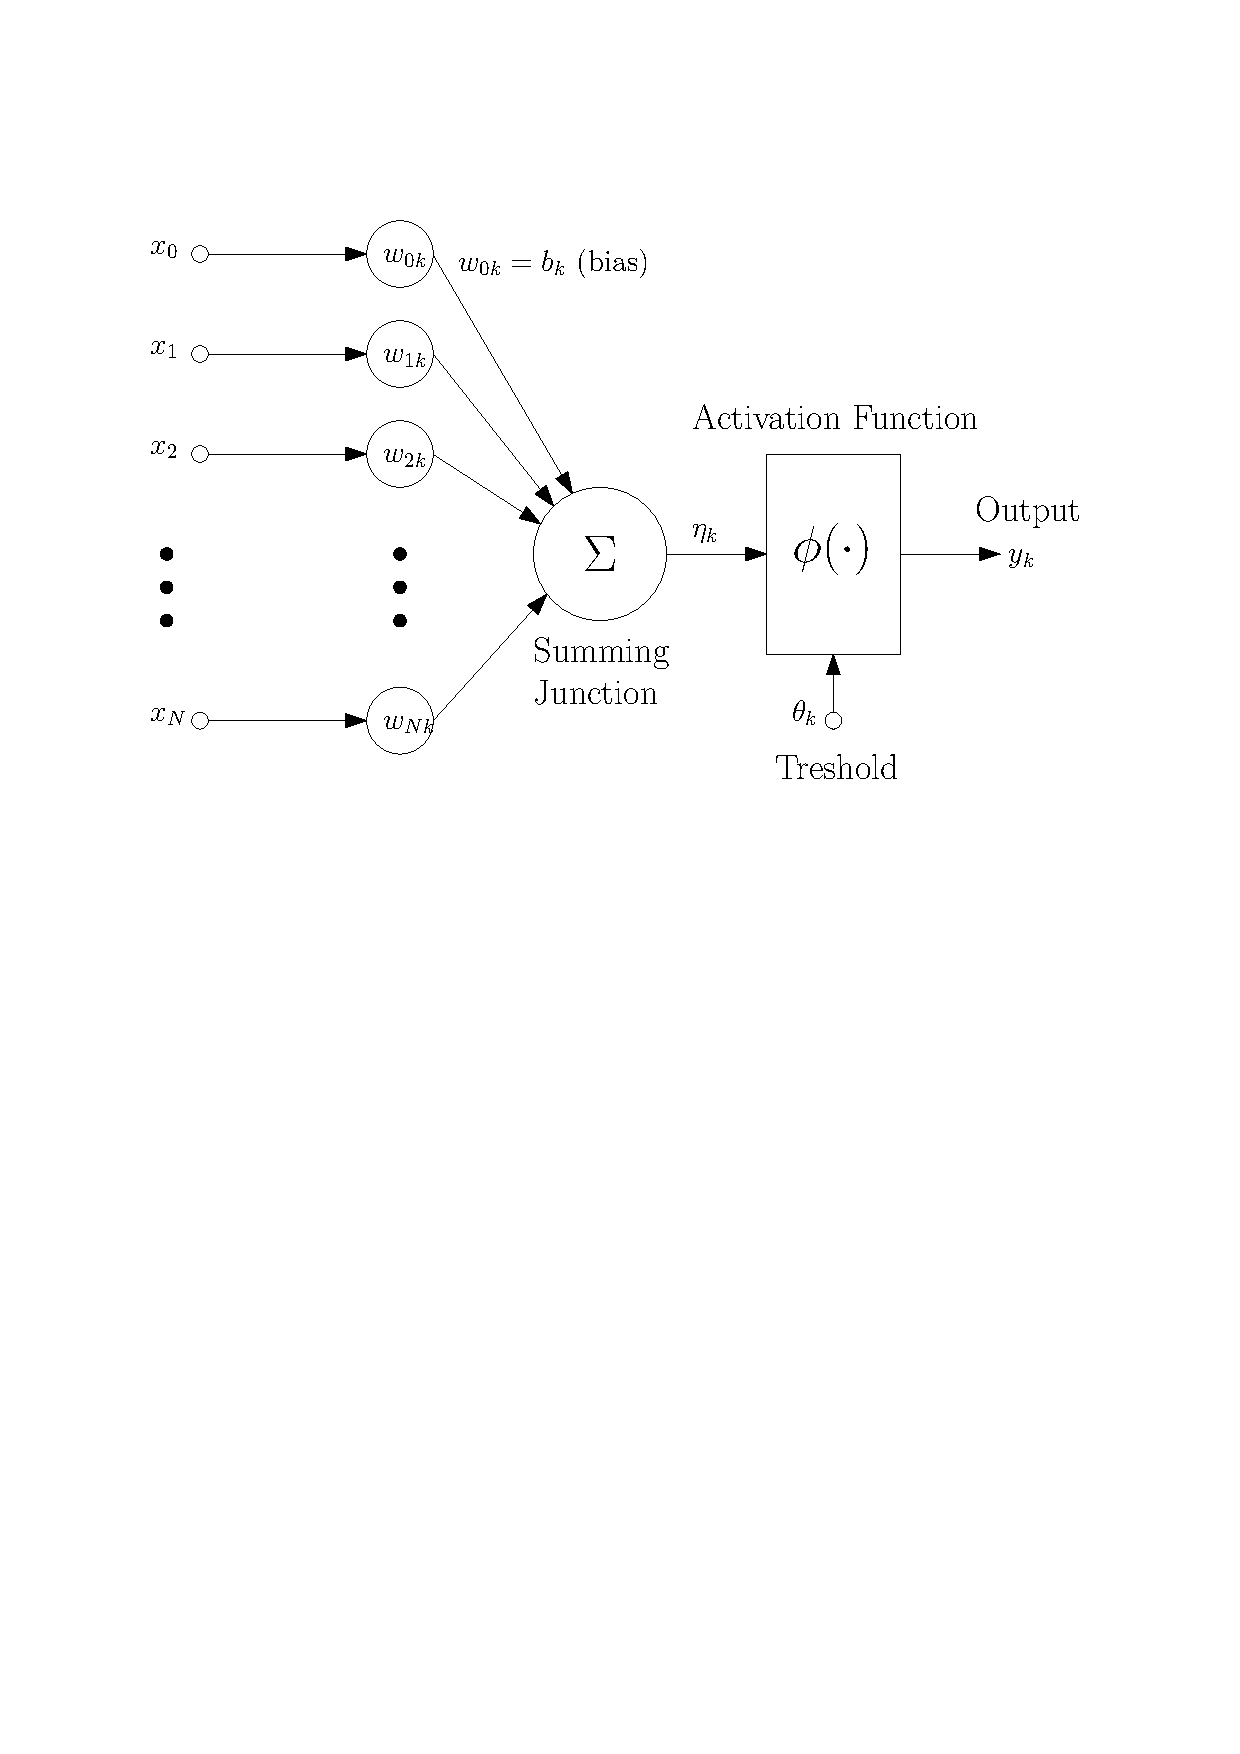
\includegraphics[width=0.6\textwidth]{img/perceptron.pdf}    
  \caption{Perceptron transforming \emph{inputs} $[x_0,\, x_1,\, \ldots,\, x_N]$ to \emph{output} $y_k$.} 
  \label{fig:perceptron}
\end{figure}

The whole transformation of the input vector to the output activation could be written as follows: 
\begin{equation}
\label{eq:perceptron} 
y_k =
\left\{
	\begin{array}{ll}
		1 & \mbox{if } \phi(\sum_{i=0}^N x_iw_{ik}) > \theta_k \\
		0 & \mbox{otherwise}
	\end{array}
\right.
\end{equation} 

Equation~\ref{eq:perceptron} describes a simple \emph{binary treshold perceptron}. One could observe that the binary perceptron divides the vector space $\mathbb{R}^N$ by a $(n-1)$--dimensional hyperplane. This behaviour was studied by~\citet{rosenblatt1958perceptron}. Now we see the importance of bias which is the absolute term in the equation of the hyperplane. \label{sec:linear-sep} This leads to the fact that for one perceptron is impossible to classify non--\emph{linearly separable} vectors. 

\paragraph{Continuous perceptron.}
We put additional constraints for the activation function $\phi : \mathbb{R} \mapsto (0,1)$ that $\phi$ is differentiable, monotonously increasing and satisfying two asymptotic conditions $t(-\infty)=0$ and $t(\infty)=1$.  Usually, the activation function is realized by the logistic function $\frac{1}{1 + \exp{-\eta}}$. To allow real numbered results from the range $(0,1)$, we drop the treshold function and simply output $\phi(\eta_k)$. 

\paragraph{Learning.} 
The goal of a perceptron is to \emph{learn} the mapping given by the set $T = \{(X^j, t_j)\}$ of pairs, where $X^j$ is the input vector $(x_{j0},x_{j1}, \ldots, x_{jN})$ and $t_j$ is the corresponding target. It could be formalized as minimizing the error function: 

\begin{equation}
\label{eq:perceptron-error} 
E = \sum_{k=1}^{N} \frac{1}{2}(t_k-y_k)^2.
\end{equation} 

A straightforward method for the network to minimize the error function \ref{eq:perceptron-error} is simply updating weights according to the partial derivates of the error function: 

\begin{equation}
\label{eq:perceptron-learning} 
\frac{\partial E}{\partial w_{ik}} = (t_k - y_k)\phi'(\eta_k)x_i = (y_k - t_k)y_k(1 - y_k)x_i,
\end{equation} 
which gives us the \emph{update rule} written as: 
\
\begin{equation} 
\label{eq:perceptron-learning-rule} 
\Delta w_{ik} = \lambda (t_k - y_k)y_k(1 - y_k)x_i,
\end{equation} 
where $\lambda$ is the \emph{learning rate}. 

Using the learning rule~(\ref{eq:perceptron-learning-rule}) and the following \emph{training} process the perceptron is able to \emph{learn}: 
%TODO check algorithm 
\begin{algorithm}[H]
  \begin{algorithmic}
    \For{$epoch = 1$ to $Epoch_{\rm max}$} 
      \ForAll{$(X^j, t_j)$ in $T$} 
        \State $y_j \gets \phi(\sum_{i=0}^N x_iw_{ik}) > \theta_k$
        \For{$i=0$ to $N$} 
          \State $w_{ij} \gets w_{ij} + \lambda (t_k - y_k)y_k(1 - y_k)x_i$
        \EndFor
      \EndFor
    \EndFor
  \end{algorithmic}
  \caption{Perceptron learning. Applying the \emph{weight update rule}~\ref{eq:perceptron-learning-rule} in loop for each sample in $T$. One main loop is called \emph{epoch}.}  
  \label{alg:perceptron-learning}
\end{algorithm} 

 
\label{sec:perceptron} 

\input{theory-mutilayer}

\subsubsection{Recurrent Networks}
\label{sec:theory-recurrent} 

Recurrent networks arise problems with computing their activations. For example imagine a cycle of neurons. That means that output of a particular unit could affect its input. Therefore the activations in general couldn't be computed only by one forward pass. This introduces real--valued dynamic systems for computing the activations. We can observe that it holds that $\frac{\partial\eta}{\partial t} = 0$ for the activations of neurons in the fixed point state. There are several approaches solving these dynamic systems and deriving the learning rule \cite{pineda1987generalization, pearlmutter1989learning, williams1989learning, elman1990finding, haykin1994neural}. 

\begin{figure}[H]
  \centering
  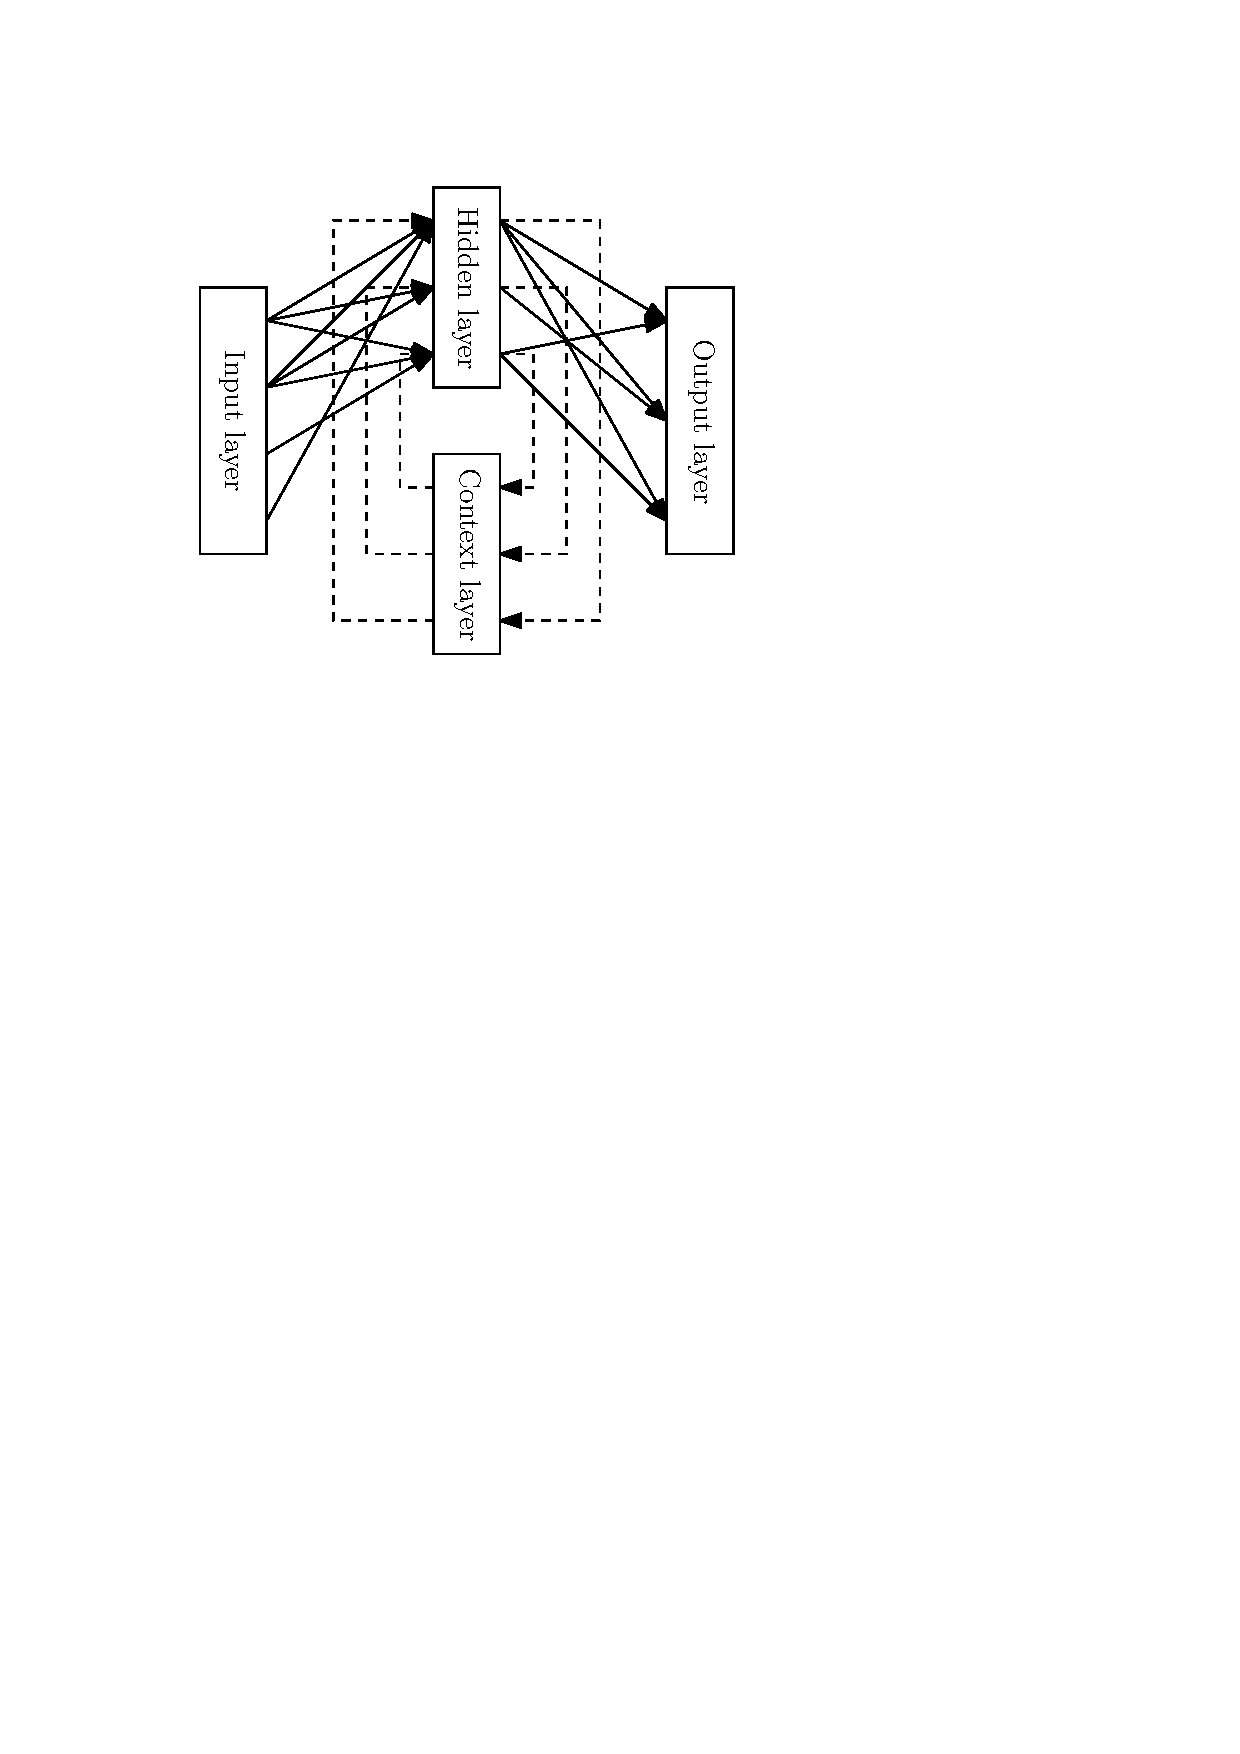
\includegraphics[width=0.4\textwidth]{img/models-recurrent.pdf}    
  \caption{Simple Recurrent network designed by \citet{elman1990finding}. Image inspiration from \citet{haykin1994neural}.} 
  \label{fig:theory-recurrent}
\end{figure}

An \emph{iterative method} is used by \citet{movellan1990contrastive} for computing activations. In the first step the input neurons have activations equal to the input vector and the other neurons have zero activation. In the next steps activations from the last step are used to compute activation in this step as shown in equation~\ref{eq:theory-recurrent-activation}: 
\begin{equation}
  \label{eq:theory-recurrent-activation} 
  \eta_i(t+1) = \phi(\sum_j w_{ji}\eta_i(t)
\end{equation}
This rule is iterated while the activation are settled. For particullar symmetric network it could be proved that activations will converge \citep{o1996bio}. For more general networks a dynamic system based on rule~\ref{eq:theory-recurrent-activation} could be derived and a fixed point solution could be found by solving a set of non--linear equations (TODO ref). \citet{movellan1990contrastive} proposes using the method of simulated annealing \citep{kirkpatrick1983optimization,vcerny1985thermodynamical} to improve the learning rule and to avoid settling the network in a local minima. We experimented with the iterative method for a two--way GeneRec \ref{sec:our-bal-recirc}. 

 

\subsubsection{Hopfield Networks}
\label{sec:theory-hopfield}

A \emph{Hopfield network} \citep{hopfield1984neurons} is a network with arbitrary connections defined only by one weight matrix $W$. Some of the units are chosen as the \emph{input units} which have stable activations for a given input pattern. We can treat a Hopfield network as a Recurrent neural network. A Hopfield network comes with an continuous error function for which usually the following function is chosen: 
\begin{equation}
  \label{eq:theory-hopfield-error}
  E = -\frac{1}{2}\sum_i\sum_ja_iw_{ij}a_j
\end{equation} 
where $a_i$ is the activation of the $i$-th unit. The aim of the network is to settle the activations so that $E$ settles in a global minimum. Activation for the $i$-th unit is computed based on the following differential equation \citep{hopfield1984neurons}: 
\begin{equation}
  \label{eq:theory-hopfield-activation}
  \frac{\partial a_i}{\partial t} = \alpha(-a_i + \phi(\eta_i)).
\end{equation} 
where $a^T = [a_1,\ldots,a_n]$ is the activation vector, $f_i$ is bounded, monotically increasing, differentiable activation function.

It could be proven for equation~\ref{eq:theory-hopfield-activation} that if the weights are symmetric, i.e. $w_{ij} = w_{ji}$, the activations will settle in the minimal error state defined by~\ref{fig:theory-hopfield-activation} \citep{hopfield1984neurons}. This learning rule is typically used in \emph{interactive activation networks} studied by \citet{grossberg1978theory, mcclelland1981interactive}. 

 
